\chapter{Research Problem and Survey}
% Survey of static hover, multirotor control and relevant topics}
% Transcribe Antonio Franchi's Talk

% (Dexterous Hexrotor)

\begin{figure}[H]
        \centering
        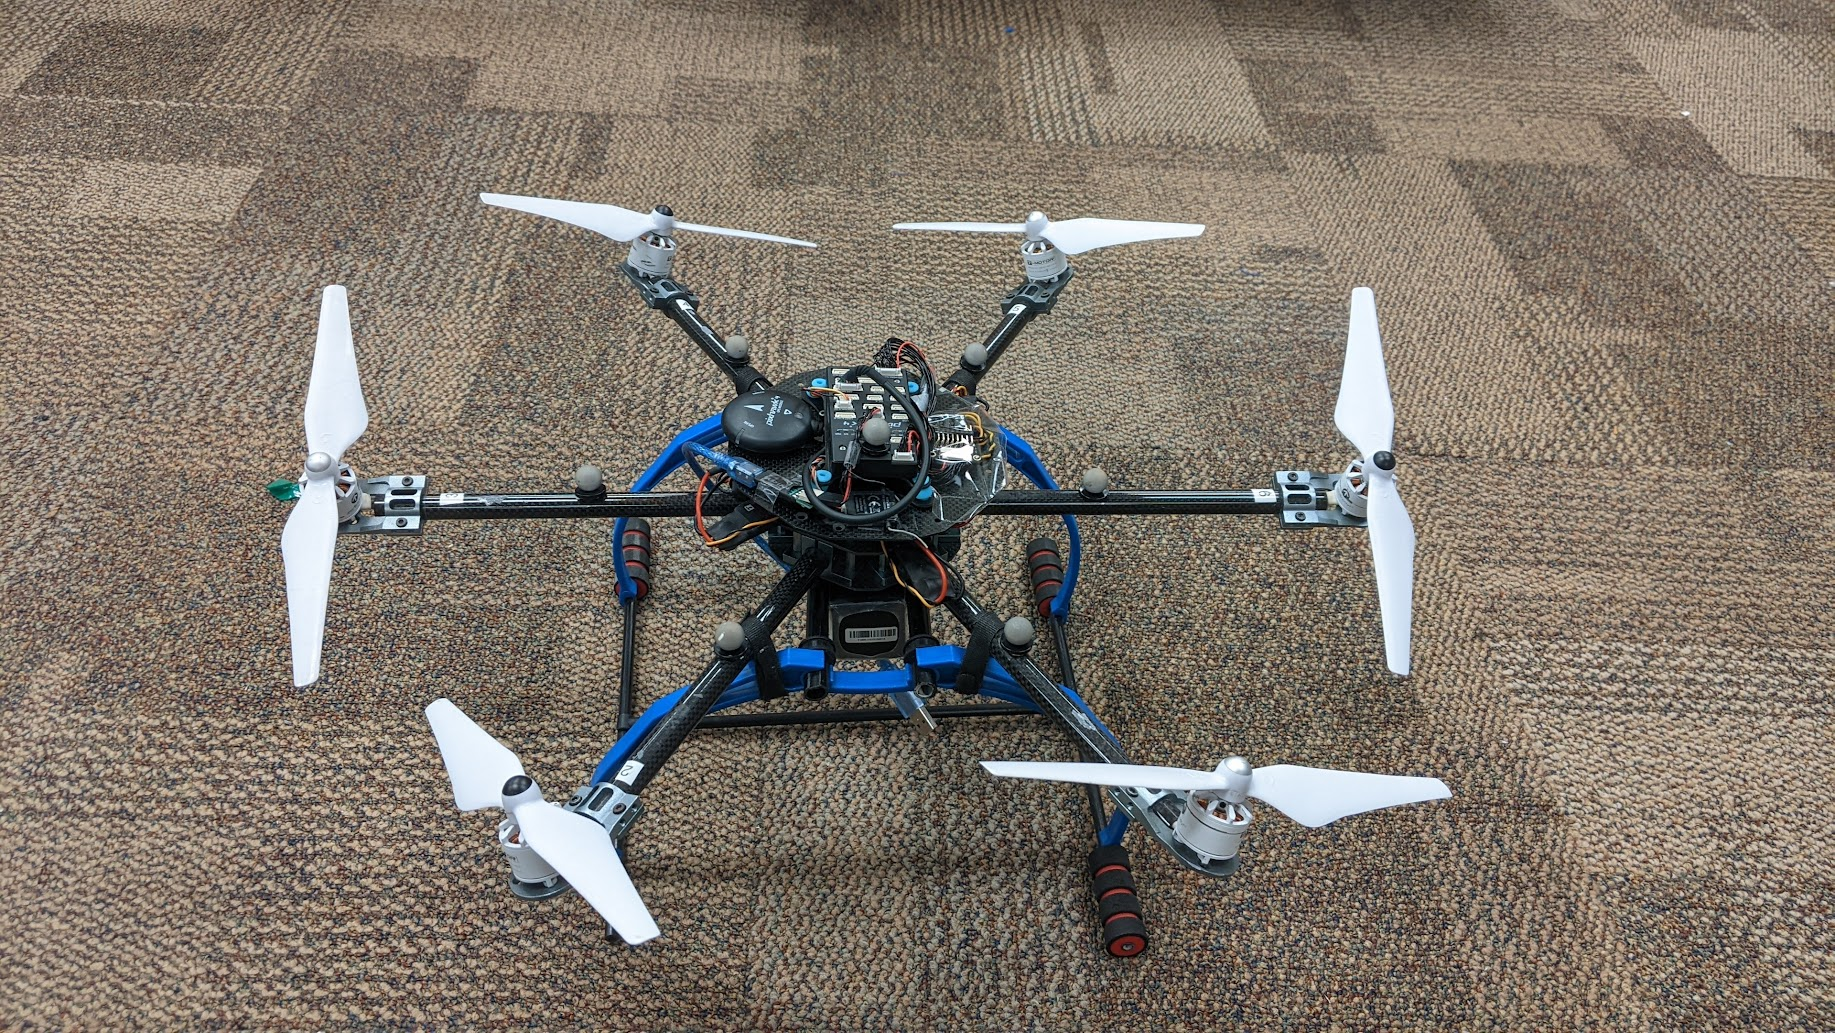
\includegraphics[width = 0.49\textwidth]{Part2/figs/1_figs/drone.jpg}
        \caption{Tilted winged hexrotor (Dexterous Hexrotor)}
        \label{fig::drone}
\end{figure}


\par The fully actuated designs of unmanned aerial vehicles (UAVs) have gained a lot of prominence over recent years for
aerial manipulation (\cite{ding2021design}, \cite{ryll20176d}). Dexterous hexrotor (figure-\ref{fig::drone}) is one such
design with applications in physical interactions with structures (\cite{jiang2017estimation}). A notable design feature
includes tilted propellers allowing independent control over the six degrees of freedom in a limited region of the state
space. The rotational inertia and mass of the large propeller blades result in actuator dynamics with time-scales
comparable to that of the dynamics of the drone effecting the performance in application of precise and controllable
forces (\cite{hamandi2021design}). In fact, the survey of \cite{hamandi2021design} noted gaps in the literature coverage
regarding theoretical analysis of actuation limits for multi-rotor UAVs.

\par The early research (2000s) in control of multirotors was primarily focused on stability and trajectory tracking in the under-actuated case. Such designs were proved to be not differentially flat but only the approximations \cite{Koo1998}. Thus, the tracking error is bounded but not asymptotically zero. The control structure primarily involves feedback linearization \cite{Mokhtari2004} or back-stepping designs \cite{Mistier2001} on transformed inputs to the system in the form of total wrench on the drone. The singularity associated with the euler angels has been overcome by using alternate parametrization for the attitude like quarternions \cite{Tayebi2006}, Lie Groups $SO(3)$ (3D rotation group)\cite{canYang} and Modified Rodrigues Parameters (MRPs) \cite{crassidis1996attitude}, etc. The primary sensor used for attitude feedback were accelerometers, gyroscopes collectively packaged as IMUs (Inertial Measurement Units) \cite{Martin2010}.

\par On the multirotor design side, several new configurations were proposed (in 2010s) including designs with changing tilt and cant angels of the propellers. Studies have shown that introducing tilt and cant angles can make the multirotors robust to actuator faults \cite{Rajappa2015}. Such designs have also been used in the area of aerial manipulation (\cite{Tognon2019},\cite{Nava2020}, \cite{lulu1}, \cite{lulu2}) where the multirotors are used for generating contact forces in a particular direction.

\par The actuator fault detection has been an important area of research in this space since the beginning \cite{6935563}. Most of the research was focused on indirectly estimating the thrust generated using observer designs such as nonlinear Thau observer \cite{hasan2018model}, etc. Other prominent method involves the use of the vibration signals due to propeller damage to detect the fault \cite{puchalski2022actuator}, \cite{thanaraj2023actuator}. These methods have proven adequate for detecting faults but lack the capacity of isolating the fault to on particular actuator.

\par One area of development that garnered less attention is the effect of propeller angular momentum on the tracking
performance in the case of fully actuated designs. The angular momentum introduces second order disturbance effects that
are justifiably neglected in the planar configurations of early studies as the tracking error can only bounded in those cases (Differential Flatness). The latter designs with tilted rotors do not suffer the same. The importance of the propeller angular momentum in the case of large propellers is demonstrated in the next section.

\par The tilted-rotor designs enable actuator redundancy which can be taken advantage of through static hover\cite{Bicego2020}. The study \cite{Michieletto2018} presents the class of designs which demonstrate such capabilities.

\par The goal of the present work is three-fold:
\begin{enumerate}
        \item Develop actuator fault detection methodology using RPM feedback and set membership techniques and demonstrate using the experimental setup.
        \item Use the propeller RPM feedback for compensating for the propeller's angular momentum in the unbalanced cases.
        \item Develop control designs for static hover of the tilted-winged hexrotor (Dexterous Hexrotor) and demonstrate through simulation studies.
\end{enumerate}

\section{Effect of propeller angular momentum}
\begin{figure}[h]
    \begin{minipage}{0.49\textwidth}
        \begin{figure}[H]
            \centering
            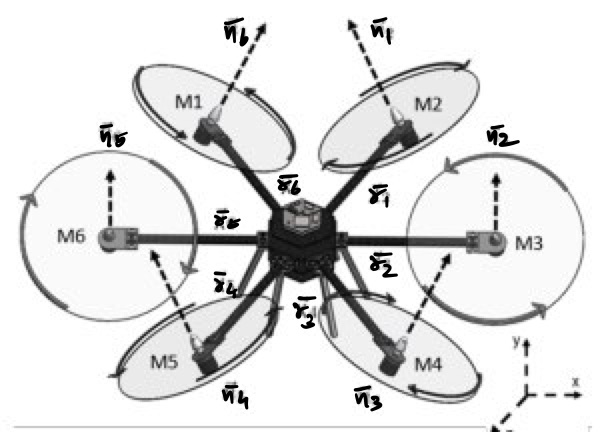
\includegraphics[width = 0.9\textwidth]{Part2/figs/1_figs/prop_momentum/hex_copt-1.jpg}
        \end{figure}
    \end{minipage}
        \begin{minipage}{0.49\textwidth}
        \begin{figure}[H]
            \centering
            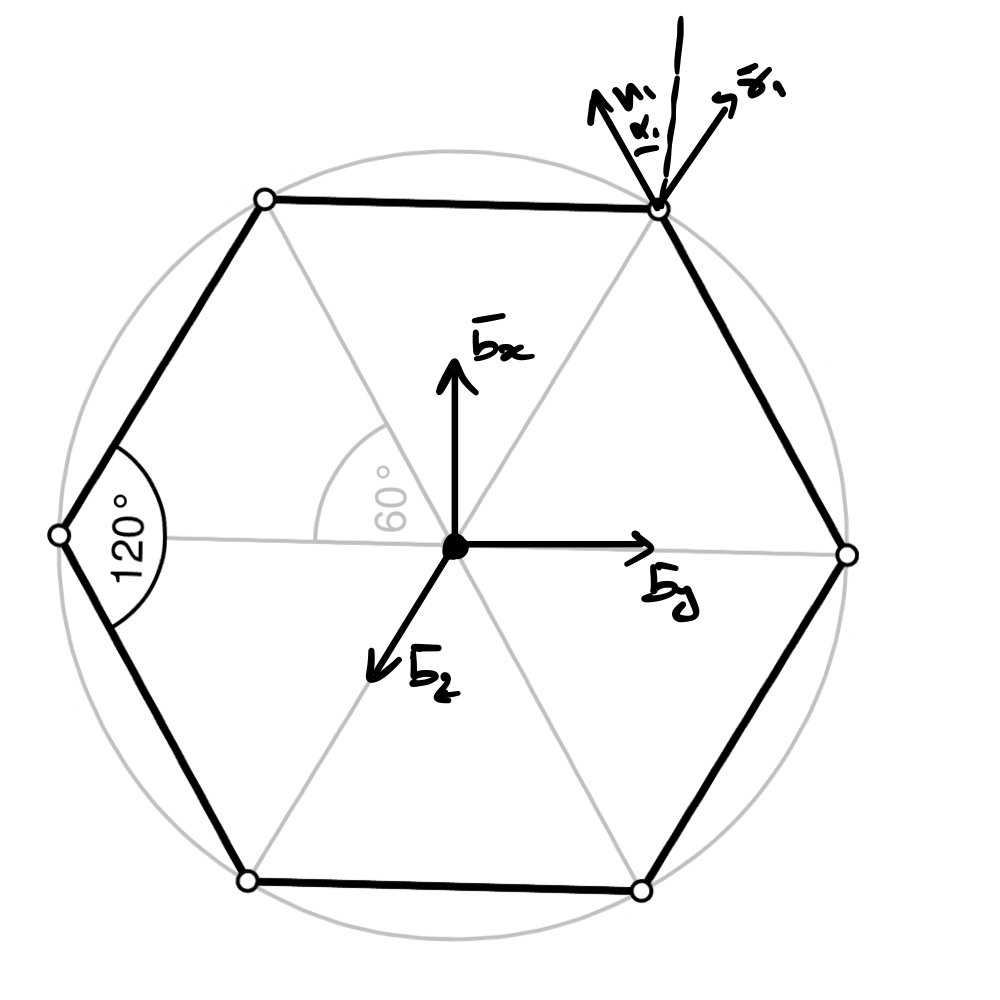
\includegraphics[width = 0.8\textwidth]{Part2/figs/1_figs/prop_momentum/hex_copt-2.png}
        \end{figure}
    \end{minipage}
\end{figure}
%
\subsection{Propeller angular velocity vectors}
Let, $b$ be the body-frame with $\{\pmb{b_x \, b_y \, b_z}\}$ as 3 mutually perpendicular right-handed unit vectors shuch that $\pmb{b_z}$ points downwards (in the direction of gravity), $\pmb{b}_x$ point forward and $\pmb{b}_y$ such that they form the right-handed system. let, $\pmb{n}_i$ be the unit vectors pointing 'upwards' perpendicular to the rotor-plane of $i^{th}$ propeller and $\pmb{r}_i$ be the radial vectors pointing outwards along the $i^{th}$ propeller shaft. the propeller tilt-angle $\alpha_i$ is conisdered positive along $\pmb{r}_i$, i.e., radially outwards.
\begin{align*}
   \therefore \alpha_i &= (-1)^{i} \alpha \qquad (\alpha_1 = -\alpha, \; \alpha_2 = \alpha \hdots) \\
   \implies \cos \alpha_i &= \cos \alpha  = c_{\alpha} \quad and\\
   \sin \alpha_i &= (-1)^{i} \sin \alpha = (-1)^{i} s_{\alpha}
\end{align*}
%===
Let, $\gamma_i$ be the angle of the $i^{th}$ propeller shaft along $\pmb{b_z}$ (clockwise), i.e.,
\begin{figure}[H]
    \begin{minipage}{0.49 \textwidth}
            \begin{align*}
            \gamma_i &= \frac{i\pi}{3} - \frac{\pi}{6} = (2i-1)\frac{\pi}{6}\\
            \implies \pmb r_i &= \cos \gamma_i \pmb b_x + \sin \gamma_i \pmb b_y
            \end{align*}
    \end{minipage}
    \begin{minipage}{0.49 \textwidth}
        \begin{table}[H]
            \centering
            \begin{tabular}{c c c c }
                \hline \hline
                $i$ & $\gamma_i$ & $c_{\gamma_i}$ & $s_{\gamma_i}$ \\ \hline \hline
                $1$ & $\frac{\pi}{6} = 30^o$   & $\frac{\sqrt{3}}{2}$ & $\frac{1}{2}$ \\
                $2$ & $\frac{\pi}{2} = 90^o$   & $0$ & $1$ \\
                $3$ & $\frac{5\pi}{6} = 150^o$ & $-\frac{\sqrt{3}}{2}$ & $\frac{1}{2}$ \\
                $4$ & $\frac{7\pi}{6} = 210^o$ & $-\frac{\sqrt{3}}{2}$ & $-\frac{1}{2}$ \\
                $5$ & $\frac{3\pi}{2} = 270^o$ & 0 & $-1$ \\
                $6$ & $\frac{11\pi}{6} = 330^o$& $\frac{\sqrt{3}}{2}$ & $-\frac{1}{2}$ \\
                \hline \hline
            \end{tabular}
        \end{table}
    \end{minipage}
\end{figure}
%===
We have the propeller normals in body-frame:
\begin{align*}
    \pmb{n}_i &= -\cos \alpha_i \pmb{b}_z + \sin \alpha_i ( \pmb b_z \times \pmb r_i)\\
    &= -c_{\alpha} \pmb b_z + (-1)^{i} s_{\alpha}( \cos \gamma_i \pmb b_y - \sin \gamma_i \pmb b_x) \qquad
    [\because ( \pmb b_z \times \pmb r_i) = \pmb b_z \times (\cos \gamma_i \pmb b_x + \sin \gamma_i \pmb b_y)]\\
    %---
    &= -(-1)^i s_{\alpha} s_{\gamma_i} \pmb b_x + (-1)^{i} s_{\alpha} c_{\gamma_i} \pmb b_y - c_{\alpha} \pmb b_z
\end{align*}
$$\therefore \pmb{n}_i = \begin{bmatrix}
    \underbrace{(-1)^{i+1} s_{\alpha} s_{\gamma_i}}_{n_{ix}} &
    \underbrace{(-1)^{i} s_{\alpha} c_{\gamma_i}}_{n_{iy}} &
    \underbrace{- c_{\alpha}}_{n_{iz}}
\end{bmatrix} \begin{bmatrix}
    \pmb b_x \\ \pmb b_y \\ \pmb b_z
\end{bmatrix}
$$
Thus, using the above definitions, we have the angular velocity vecotor of $i^{th}$ propeller:
$${}^B\pmb \omega_i = (-1)^{i} \omega_i \pmb n_i \qquad \text{where, }\omega_i \geq 0 \quad \forall i = 1, 2, \hdots, 6$$
%===
% \subsection{Attitude and euler angles $(\phi, \theta, \psi)$}
% Let, $\{ \pmb a_x, \pmb a_y, \pmb a_z \}$ be three mutually perpendicular,
% right-handed vecotors in intertial frame $R$, such that they coinside with
% $\{ \pmb b_x, \pmb b_y, \pmb b_z\}$ respectively when $\pmb b_z$ is aligned to
% acceleration due to gravity $\pmb g$.
% Let, $\{ \pmb l_x, \pmb l_y, \pmb l_z\}$ be mutually perpendicular,
% right-handed directed line segments along $\{ \pmb a_x, \pmb a_y, \pmb a_z \}$
% initally.
%
% The 'attitude' of B relative to $\{ \pmb a_x, \pmb a_y, \pmb a_z \}$ can be
% specified interms of  three angles $\phi, \theta, \psi$ generated as follows:
% Performing successive right handed rotations of amount $\phi$ about $\pmb l_x$,
% $\theta$ about $\pmb l_y$ and $\psi$ about $\pmb l_z$ results in $\{ \pmb l_x,
% \pmb l_y, \pmb l_z\}$ coinside with $\{ \pmb b_x, \pmb b_y, \pmb b_z\}$.
%
% The above successive rotations can be represented as the following rotation matrics:
% \begin{align*}
%     R_{\phi} = \begin{bmatrix}
%         1 & 0 & 0\\
%         0 & c_{\phi} & s_{\phi}\\
%         0 & -s_{\phi} & c_{\phi}
%     \end{bmatrix} \qquad
%     R_{\theta} = \begin{bmatrix}
%         c_{\theta} & 0 & -s_{\theta}\\
%         0 & 1 & 0 \\
%         s_{\theta} & 0 & c_{\theta}
%     \end{bmatrix} \qquad
%     R_{\psi} = \begin{bmatrix}
%         c_{\psi} & s_{\psi} & 0\\
%         -s_{\psi} & c_{\psi} & 0\\
%         0 & 0 & 1
%     \end{bmatrix}
% \end{align*}
% $$\implies [\pmb b_x, \pmb b_y, \pmb b_z]^T = R_{\psi}R_{\theta}R_{\phi} [\pmb a_x, \pmb a_y, \pmb a_z]^T$$
% We have,
% $$R_{\psi}R_{\theta}R_{\phi} =\displaystyle \left[\begin{matrix}\cos{\left(\psi
% \right)} \cos{\left(\theta \right)} & \sin{\left(\phi \right)}
% \sin{\left(\theta \right)} \cos{\left(\psi \right)} + \sin{\left(\psi \right)}
% \cos{\left(\phi \right)} & \sin{\left(\phi \right)} \sin{\left(\psi \right)} -
% \sin{\left(\theta \right)} \cos{\left(\phi \right)} \cos{\left(\psi \right)}\\-
% \sin{\left(\psi \right)} \cos{\left(\theta \right)} & - \sin{\left(\phi
% \right)} \sin{\left(\psi \right)} \sin{\left(\theta \right)} + \cos{\left(\phi
% \right)} \cos{\left(\psi \right)} & \sin{\left(\phi \right)} \cos{\left(\psi
% \right)} + \sin{\left(\psi \right)} \sin{\left(\theta \right)} \cos{\left(\phi
% \right)}\\\sin{\left(\theta \right)} & - \sin{\left(\phi \right)}
% \cos{\left(\theta \right)} & \cos{\left(\phi \right)} \cos{\left(\theta
% \right)}\end{matrix}\right]$$
%===
% \subsubsection{Angular velocity vector of the body ($\Omega$)}
% %===
% We have the instantaneous angular velocity of the body as:
% \begin{align*}
%     {}^R\pmb \Omega^B &= \dot \phi \pmb l_x + \dot \theta \pmb l_y + \dot \psi \pmb l_z\\
% \end{align*}
% The vectors $\{ \pmb l_x, \pmb l_y, \pmb l_z\}$ can be written in terms of $\{ \pmb b_x, \pmb b_y, \pmb b_z\}$ as follows:
% \begin{align*}
%     \pmb l_z &= \pmb b_z \qquad [\because R_{\psi} \text{ is about } \pmb l_z]\\
%     %===
%     \pmb l_y &= R_{\psi}^T [2, :]\begin{bmatrix}
%     \pmb b_x \\ \pmb b_y \\ \pmb b_z\\
% \end{bmatrix} = s_{\psi} \pmb b_x + c_{\psi} \pmb b_y\\
%     %===
%     \pmb l_x &= [R_{\theta}^T R_{\psi}^T][1,:] \begin{bmatrix}
%     \pmb b_x \\ \pmb b_y \\ \pmb b_z\\
% \end{bmatrix} = \begin{bmatrix}
%     c_{\theta}c_{\psi} & -c_{\theta}s_{\psi} & s_{\theta}
% \end{bmatrix}\begin{bmatrix}
%     \pmb b_x \\ \pmb b_y \\ \pmb b_z\\
% \end{bmatrix}
% \end{align*}
% %====
% Hence,
% \begin{align*}
%     {}^R\pmb \Omega^B &=
%         \dot \phi \begin{bmatrix} c_{\theta}c_{\psi} & -c_{\theta}s_{\psi} &
%         s_{\theta} \end{bmatrix}\begin{bmatrix} \pmb b_x \\ \pmb b_y \\ \pmb
%         b_z\\\end{bmatrix} +
%         \dot \theta \begin{bmatrix} s_{\psi} & c_{\psi} & 0
%         \end{bmatrix}\begin{bmatrix} \pmb b_x \\ \pmb b_y \\ \pmb
%         b_z\\\end{bmatrix} +
%         \dot \psi \begin{bmatrix} 0 & 0 & 1\end{bmatrix}
%         \begin{bmatrix} \pmb b_x \\ \pmb b_y \\ \pmb
%         b_z\\\end{bmatrix}
% \end{align*}
% %===
% Let,
% \begin{align*}
%     {}^R\pmb \Omega^B  &= \Omega_x \pmb b_x + \Omega_y \pmb b_y + \Omega_z \pmb b_z\\
% \end{align*}
% %===
% combaring the coefficients,
% \begin{align*}
%     \begin{bmatrix}
%         \Omega_x \\ \Omega_y \\ \Omega_z
%     \end{bmatrix}
%     &=
%     \begin{bmatrix}
%         c_{\theta}c_{\psi} &  s_{\psi} & 0\\
%         -c_{\theta}s_{\psi} & c_{\psi} & 0\\
%         s_{\theta} & 0 & 1
%     \end{bmatrix}
%     \begin{bmatrix}
%         \dot \phi \\ \dot \theta \\ \dot \psi
%     \end{bmatrix}
% \end{align*}
% %===
% Thus, the instantaneous angular velocity is purely a function of $\dot \phi , \dot \theta , \dot \psi $.
%===
\subsection{Inertial moments due to propeller angular momentum}
Let, ${}^R \pmb \Omega^B$ be the angular velocity of the drone in inertial frame. We have, angular velocity of the propeller $i$ in inertial frame:
$${}^R \pmb \omega_i = {}^R \pmb \Omega^B + {}^B \pmb \omega_i$$
Hence, angular acceleration in reference frame:
\begin{align*}
    \frac{{}^R d \pmb \omega_i}{dt} &= \frac{{}^R d}{dt}\left( {}^R \pmb \Omega^B + {}^B \pmb \omega_i \right)
    = \underbrace{\frac{{}^R d \pmb \Omega^B}{dt}}_{{}^R\pmb\alpha^B} + \frac{{}^R d{}^B \pmb \omega_i}{dt}\\
    %==
\text{Consider,} \qquad & \\
%===
    \frac{{}^R d{}^B \pmb \omega_i}{dt} &= \frac{{}^R d}{dt} (-1)^{i} \omega_i \pmb n_i
    = \underbrace{(-1)^{i} \frac{{}^R d\omega_i }{dt} \pmb n_i}_{{}^B \pmb \alpha_i} +
    (-1)^{i} \omega_i \frac{{}^R d\pmb n_i}{dt} \\
\text{We have,} \qquad &\\
    \frac{{}^R d\pmb n_i}{dt} &= {}^R \pmb \Omega^B \times \pmb n_i
    = \begin{bmatrix}
        \Omega_y n_{iz} - \Omega_z n_{iy} &
        \Omega_z n_{ix} - \Omega_x n_{iz} &
        \Omega_x n_{iy} - \Omega_y n_{ix}
    \end{bmatrix}
    \begin{bmatrix}
    \pmb b_x \\ \pmb b_y \\ \pmb b_z\\
    \end{bmatrix}
\end{align*}
%
Let, $\dot \varepsilon^T  = \begin{bmatrix} \dot \phi & \dot \theta & \dot \psi \end{bmatrix}$. We have,
%
\begin{alignat*}{3}
        \Omega_x &=  c_{\theta}c_{\psi} \dot \phi + s_{\psi} \dot \theta \qquad
        \Omega_y &&= -c_{\theta}s_{\psi} \dot \phi + c_{\psi} \dot \theta \qquad
        \Omega_z &&= s_{\theta} \dot \phi + \dot \psi\\
        n_{ix}   &=  (-1)^{i+1} s_{\alpha} s_{\gamma_i} \qquad
        n_{iy}   &&= (-1)^{i} s_{\alpha} c_{\gamma_i}  \qquad \qquad
        n_{iz}   &&= -c_{\alpha}
\end{alignat*}
%
% Calculating the individual terms:
% \begin{align*}
%     \Omega_y n_{iz} - \Omega_z n_{iy} &=
%     \begin{bmatrix}
%         \dot \phi & \dot \theta & \dot \psi
%     \end{bmatrix}
%     \begin{bmatrix}
%         (-1)^{i+1} s_{\theta} s_{\alpha} c_{\gamma_i} + s_{\psi} c_{\theta} c_{\alpha}\\
%         -c_{\psi} c_{\alpha}\\
%         (-1)^{i+1} s_{\alpha} c{\gamma_i}
%     \end{bmatrix}\\
%     %===
%     \Omega_z n_{ix} - \Omega_x n_{iz} &=
%     \begin{bmatrix}
%         \dot \phi & \dot \theta & \dot \psi
%     \end{bmatrix}
%     \begin{bmatrix}
%         (-1)^{i+1} s_{\theta} s_{\alpha} s_{\gamma_i} + c_{\psi} c_{\theta} c_{\alpha}\\
%         s_{\psi} c_{\alpha}\\
%         (-1)^{i+1} s_{\alpha} s_{\gamma_i}\\
%     \end{bmatrix}\\
%     %===
%     \Omega_x n_{iy} - \Omega_y n_{ix} &=
%     \begin{bmatrix}
%         \dot \phi & \dot \theta & \dot \psi
%     \end{bmatrix}
%     \begin{bmatrix}
%         (-1)^{i} c_{\theta}s_{\alpha} (c_{\gamma_i}c_{\psi} - s_{\gamma_i} s_{\psi})\\
%         (-1)^{i} s_{\alpha} (s_{\gamma_i} c_{\psi} + c_{\gamma_i} s_{\psi})\\
%         0
%     \end{bmatrix}
% \end{align*}
Hence,
\begin{align*}
    \frac{{}^R d\pmb n_i}{dt} &= {}^R \pmb \Omega^B \times \pmb n_i\\
    &= \begin{bmatrix}
        \dot \phi & \dot \theta & \dot \psi
    \end{bmatrix}
    \underbrace{\begin{bmatrix}
        (-1)^{i+1} s_{\theta} s_{\alpha} c_{\gamma_i} + s_{\psi} c_{\theta} c_{\alpha}
        & (-1)^{i+1} s_{\theta} s_{\alpha} s_{\gamma_i} + c_{\psi} c_{\theta} c_{\alpha}
        & (-1)^{i} c_{\theta}s_{\alpha} c_{\gamma_i + \psi}
        \\
        -c_{\psi} c_{\alpha}
        & s_{\psi} c_{\alpha}
        & (-1)^{i} s_{\alpha} s_{\gamma_i + \psi}
        \\
        (-1)^{i+1} s_{\alpha} c{\gamma_i}
        & (-1)^{i+1} s_{\alpha} s_{\gamma_i}
        & 0
    \end{bmatrix}}_{G_i}
    \underbrace{\begin{bmatrix}
    \pmb b_x \\ \pmb b_y \\ \pmb b_z\\
    \end{bmatrix}}_{\pmb b}
\end{align*}
%
The inertial moment associated with the above motion is:
\begin{align*}
    M_{g_i} =  I_p \times (-1)^{i} \omega_i \left[\dot \varepsilon^T  G_i \pmb b \right]
\end{align*}
where, $I_p$ is the moment-of-inertia matrix of the propeller.
%
\subsubsection{Result of opposing spin for diagonally opposing propellers}
%
The opposing propeller pairs from the given configuration are $(1, 4), (2, 5) \text{ and } (3, 6)$. From the above derivation of $G_i$ matrix, it can be concluded that it is same for opposing propeller paris (the $-ve$ sign difference due to $(-1)^i$ or $(-1)^{i+1}$ is compensated by the negative sign difference in $c_{\gamma_i} \text{ and } s_{\gamma_i}$ for the opposing propellers), i.e.,
$$ G_{i} = G_{i+3} \qquad i = 1, 2, 3$$

Hence, the opposing propellers create inertial moments along the same line but in opposing directions. Hence the difference in the propeller velocities will cause the inertial moments in that particular direction. Thus we have, the inertial moments resulting from the propeller velocity difference:
%
\begin{align*}
    \delta M_{g_{14}} &=   I_p \delta \omega_{14} \left[\dot \varepsilon^T  G_{1 4} \pmb b \right] \qquad \delta \omega_{14} = \omega_4 - \omega_1, \quad G_{14} = G_1 = G_4\\
    %===
    \delta M_{g_{25}} &=   I_p \delta \omega_{25} \left[\dot \varepsilon^T  G_{2 5} \pmb b \right] \qquad \delta \omega_{25} = \omega_5 - \omega_2, \quad G_{25} = G_2 = G_5\\
    %==
    \delta M_{g_{36}} &=   I_p \delta \omega_{36} \left[\dot \varepsilon^T  G_{3 6} \pmb b \right] \qquad \delta \omega_{14} = \omega_6 - \omega_3, \quad G_{36} = G_3 = G_6\\
\end{align*}
%

